\documentclass[aps,rmp,onecolumn]{revtex4-1}
\usepackage{geometry}
\usepackage{graphicx}
\usepackage{hyperref}
\usepackage{xcolor}


\newcommand{\Marco}[1]{{\color{gray}Marco: #1}}
\newcommand{\Liam}[1]{{\color{teal}Liam: #1}}

\definecolor{response}{rgb}{0.2, 0.2, 0.2}
\newcommand{\reviewer}[2]{\textbf{#1:} #2\vskip 5mm}
\newcommand{\response}[1]{{\it {\color{response}\textbf{Response:} #1}}\vskip 5mm}
\newcommand{\responsedraft}[1]{{\it {\color{purple}\textbf{ResponseDraft:} #1}}\vskip 5mm}

\title{Response to Reviewers}
\begin{document}
\maketitle

\section*{Response to reviewers}

\subsection*{Reviewer 1}

\reviewer{R1}{Bacterial evolution is driven both by local (vertical) mutation and larger scale (horizontal) genome alternations resulting in gain, loss, inversion or reassortment of genetic material. A single linear reference cannot capture this larger scale diversity, and existing graph reference structures either depend on coloured de Bruijn graphs (losing long range homology) or simplify the complex topologies by partitioning the pangenome and considering genes/loci in isolation. PanGraph provides a library and data structure to create a pangenome reference graph for closely related bacteria based on a progressive multiple sequence alignment approach.

      It is not easy to handle this sort of diversity efficiently and I was excited to read about the neat tricks employed to allow for a progressive alignment approach within reasonable resources, including parallelisation.

      This paper was clearly organised and a real pleasure to read. The niche was clearly described and demonstrated. The tests were well thought through. A lot of care had been taken to demonstrate the effects of different levels of bacterial diversity on the resulting graphs. The deliberate inclusion of P. marinus provided a clear informative demonstration of the limit of the software capabilities.

      The software was easy to install and the documentation available online is impressive.

      There was no comparison with other tools - would be appropriate if e.g. downstream mapping performance were evaluated but that is outside the scope here.\\

      On reading I had a few queries, which could perhaps be clarified further in the text.}

\reviewer{R1.1}{A pancontig is defined as a multiple sequence (sub)alignment. In line 54 you say "Pairwise graph alignment is performed by an all-to-all alignment of the pancontigs" which I interpreted to mean all sequences in the alignment vs all sequences in another alignment. You do later add that "To align two graphs, the consensus sequences of all pancontigs in both graphs are searched for homologies and aligned". Adding the word consensus in the earlier sentence might avoid confusion.}
% \Marco{changed to ``Pairwise graph alignment is performed by an all-to-all alignment of the \emph{pancontigs} consensus sequences between both graphs, and the order of pairwise alignments is determined by a guide tree." Too compressed? I could also break in two sentences and expand a bit more.}\\
% \Liam{that's clear to me.}
\response{We agree with the reviewer suggestion. The wording in Line 54 has been updated to ``all-to-all alignment of the \textit{pancontigs} consensus sequences''.}

\reviewer{R1.2}{Figure 4C: The main text talks about how to interpret this, as ~1/N for TB and a bit less compression for E. coli and K. pneumoniae where the core is a smaller fraction, but this is not so easy to interpret from the figure. Would it be possible to rescale this plot to orders of magnitude of N? Or in another way aid this reading?}
\response{We agree with the reviewer that it is important to be able visually compare the compression with the number $N$ of isolates for each species, and we thank him for the suggestion. We modified fig.~4C in the main text and fig.~4I in SI marking the value of $1/N$ for each species with horizontal lines, and updated the captions accordingly.}
% \Marco{maybe try visualizing it as deviation from "one strain" compression (1/N)? But the "maximal" compression depends not only on the sample size N but also on the gene frequency distribution. Another possible comparison might be to pangraph's estimation of the pangenome size, but again we might have different effects coming into play.}\\
% \Liam{yes, I think just adding a dashed line for 1/N for each species to the plot would aid that reading and satisfy this point.}

\reviewer{R1.3}{Figure 5 has 2 typos: pacontigs and panconting.}
% \Marco{fixed.} 

\response{The typos have been corrected.}

\reviewer{R1.4}{Throughout the text E. Coli and K. Pneumoniae etc capitalization.}
% \Marco{fixed.}
\response{The capitalization has been corrected.}

\reviewer{R1.5}{Line 213: Core pancontigs have higher than average size - is this what you would expect given that if they are core genes then they will be present in more/all of the samples so there could be more diversity due to being more sampled?}
% \Marco{here the pancontig size is the consensus sequence length. I would say that the fact that they have higher-than-average size is mostly due to synteny. Long blocks (several kbps) contain core genes that always appear in the same order, without any accessory sequence ever occurring in these regions. As opposed to accessory regions with a lot of structural diversity, that generates short fragments. But here the main message is that core blocks are well-behaved (close to N50 line in the figure), as opposed to fine-grained structural diversity, part of which contains artifacts generated by the block size limit (many short 100bp blocks). Should we show block frequency distributions in the supplementary?}\\
% \Liam{I don't understand their point on diversity - maybe they misunderstood the meaning of size. Maybe pancontig `length' is clearer? I agree with you about synteny and think this is a nice point to add here to explain the observation.}
\response{The observation that core pancontigs are longer than average was in agreement with the expectation that core genes would be more syntenic and present less structural fragmentation compared to accessory genes. In contrast, we expected most short pancontigs to be located around recombination islands, where structural variation is high across different genomes.
      We modified the line to: ``Core pancontigs having higher-than-average length. This is expected given their strong synteny and the fact that they present less structural variation across genomes compared to accessory genes.''}

\reviewer{R1.6}{Figure 6B: could you explore another way to project this data so it is not squished at the ends? I can't read off the fraction agree (shared+private) or disagree which I would like to (although at a glance this is exactly the result you want to see, so happy for it to stand if it is the best projection).}
% \Marco{maybe add mean and standard deviation as numbers on the side?}\\
% \Liam{that seems ideal.}
\response{We considered different projections and in the end decided to maintain the linear projection for ease of interpretation, but we added next to each distribution its mean and standard deviation. In this way both deviations from 0 and 1 in the first two distributions can be quantified.}

\reviewer{R1.7}{Have you tried running PanGraph on more than 300 references? I'd love to see another order of magnitude (not necessary for the paper, just curiosity)}
% \Marco{not really, I never tried on ~500 or ~1000 strains. I could try but would not consider this a priority.}\\
% \Liam{agree that it's not necessary.}
\response{The biggest dataset we tried PanGraph on is a collection of 500 E.coli isolates. We used minimap2 as alignment kernel, asm20 sensitivity and values of $\alpha = 100$, $\beta=20$. This took 18 hours and 12 minutes to complete and had maximum memory usage of 17Gb.}

\reviewer{R1.8}{Discussion: Do you know of/have you tried any mapping approaches which could take this reference as an input. Could you touch on the downstream applications of this graph structure? I would like to see discussion of how the graph can be used downstream - e.g. touching on what software can be used to map/align to such a data structure? Or how it can be used to analysis genome structure.}
\Marco{other than explicitly exporting block sequences and mapping to those, we do not really using the pangenome graph as a reference against which to map new strains... But we could expand the discussion with more ideas on applications to study pangenome organization and evolution. For software for further analysis and exploration I have \href{https://github.com/mmolari/pypangraph}{this package} to explore and interact with graphs in python, but not sure it's worth mentioning.}\\
\Liam{Some ideas that could be mentioned. (1) I think one obvious (bad!) use would be to take the core blocks and map reads to those as a `core reference'. (2) I know pandora has \href{https://github.com/iqbal-lab-org/make_prg/}{\texttt{make\_prg}} which will construct a `pangenome reference graph' from a set of aligned sequences - I didn't try it on pangraph output. (3) For genome structure, exploring `hotspots' in the graph as \href{https://www.nature.com/articles/s41467-017-00808-w}{this paper} does could be done using in/out degree of pancontigs.}

\reviewer{R1.9}{Supplementary Information: simulation - could you comment on how/if homologous recombination is included in this model e.g. within a gene.}
% \Marco{homologous recombination is not implemented directly in the model. Only sequence transfer between strains. Genes are not explicitly modeled in the simulation.}\\
% \Liam{think just adding a comment in the SI saying this is required.}
\response{Homologous recombination is not directly included in our simulated data generation procedure. We only simulate transfer of sequence between two genomes but this transfer is not based on homology. Moreover we simulate sequence evolution without a notion of genes. This is now specified in SI section II. To avoid confusion we also changed ``Horizontal Gene Transfer'' to ``Horizontal Sequence Transfer''.}

\reviewer{R1.10}{Supplementary Information C: You comment that the use of null energy parameters results on average in "more and shorter pancontigs" but also that they result in more diverged sequences being merged into the same pancontig. Why is a more diverse pancontig more likely to become fragmented?}
% \Marco{I think that basically the reason is that merging more distant paralogs/orthologs can fragment more the graph. Maybe we could explain this more explicitly in the text.}\\
% \Liam{makes sense and explaining this reasoning sounds good.}
\response{We use the pseudo-energy defined in eq.~(1) as an heuristic to decide whether a homologous match detected by our aligner should result in a merge between two pancontigs, depending on the match length and on sequence divergence. In particular any choice of $\beta$ would result in no merges between sequences with divergence higher than $1/\beta$. Setting $\beta=0$ instead does not impose a divergence limit on merges, other than the one intrinsically set by the aligner sensitivity. In this sense the choice of null energy parameter results in more diverged sequences being merged into the same pancontig. A consequence of more merging is also more fragmentation of the graph, since the merging of a homologous section of two pancontigs often requires splitting them in chunks. Therefore we expected that the choice of null energy parameters would lead to shorter pancontigs, and alignments containing more diverged sequences.
      To make this reasoning more explicit we added section I in the SI to better explain the merging procedure and the effect of tuning the pseudo-energy parameters.}


\subsection*{Reviewer 2}

\reviewer{R2}{In this paper, Noll et al set out to make a novel contribution to the pangenomics field. As it stands prior to this work, pangenomics splits into 3 different approaches

      \begin{enumerate}
            \item People working in human genomics are working to develop a graph human reference. The challenge there is one of scale - large genomes with comparatively small pan-genomes (in the classical/bacterial sense) except for some devilish mess at the centromeres. This is essentially a subfield of its own focussed on the needs of human and clinical genetics.

            \item People working in bacterial genomics who do reference-based SNP calling plus gene-presense/absence, or more recently building gene order graphs (panaroo) and even gene calling /detection on graphs (ggcaller).

            \item People breaking the pan-genome up into a collection of orthologous blocks and then building a collection of pan-genome graphs (pandora), at the cost of losing order information.
      \end{enumerate}


      Noll et al set out to build a representation which combines a global pan-genome with local MSAs, and to do so in a way which scales well, and which provides easy to use visualisations. It is an ambitious aim, and in my opinion this is great work. They have developed something noone else has (see enumeration above), and the paper does a good job of describing and then evaluating their work - they are to be congratulated. This tool is sure to be extremely useful, and very valuable to the community. I have no serious reservations about the quality or calibre of the work, i admire it greatly.\\

      Nevertheless, there are a number of clarifications which need to be addressed before the paper is suitable for publication.}

\subsubsection*{Major Issues}

\reviewer{R2.1}{Line 46: when you say "PanGraph transforms an arbitrary set of genomes into a graph that simultaneously compresses the collection of sequences and exhaustively summarizes both the structural and nucleotide-level polymorphisms." - I am a bit unclear on how the nucleotide level variation is summarised. The paper is a bit hand-wavey about this. When i dug around on github , i found this helpful page \url{https://neherlab.github.io/pangraph/tutorials/tutorial_2/} Which answers and raises questions. So, my question: for each pancontig (which i think is the same as a block), i think what you do is infer a consensus (what is this? majority base at each position but somehow also choose an allele when there is an indel?), and then you describe the other alleles in the MSA as edits from this? You surely do not do all pairwise descriptions of SNPS, right? On that same webpage you have a section on ``block consensus to node alignment'' - how do you choose the order of alleles here? This is all valuable information and it would be great to have it in the supplementary or main methods somewhere.}
% \Marco{this point was also raised by R3. Mutations are always represented as variation on the consensus. The way consensus is propagated during graph merging might require more explanation. Maybe we could add a section in the supplementary with a somewhat more detailed description of the algorithmic steps we perform when merging two graphs? In the code \href{https://github.com/neherlab/pangraph/blob/e1c11012a3d19975d4b1dc61b1af3eb3949f7cd2/src/block.jl\#L1274}{this part} takes care of merging alignments between two blocks with only small (i.e. below cutoff) insertions and deletions. In short what we do is stitch the two alignments together using the cigar string as a guide, and re-compute the consensus on the newly-obtained alignment. This ensures that the consensus agrees with the majority of sequences in the alignment, but does not solve the full multiple sequence alignment problem. However we also provide the ``polish'' step for this, that can be executed after graph creation. This will take care of refining the block alignments.}\\
% \Liam{I think a `narrative section' in the supplementary describing this in brief sounds great.}
\response{In our pangenome graph representation each pancontig encodes an alignment using a consensus sequence, and encoding each line as variations over the consensus. The consensus sequence is defined using the majority rule on the alignment and is updated at each pancontig merge. Each line in the alignment is then only described as variations over this consensus (mutations, insertions and deletions).\\
      To make this more clear we introduced section I in SI, in which we explain in more detail the merging procedure and how the consensus sequence is updated. We also refer to the documentation page mentioned by the reviewer. Moreover, to avoid ambiguity we also avoided referring to pancontigs as ``blocks'' in the main text.}

\reviewer{R2.2}{Line 61: I agree and understand how each sequence can be sketched in linear time. I don't follow how you calculate all pairwise intersections through sorting the list of minimizers, nor do i see how this ends up being log-linear. For each genome, you can sort it's minimizers in nlog(n) (ie log linear), where n ~genome length. How do you get all pairwise distances from that without another multiplier of n?}
% \Marco{in the text we write that ``the pairwise distance matrix is estimated in a time that increases log-linearly in the \textbf{total length} of sequence that is analyzed.'' This might generate some confusion since the scaling depends both on the number of genomes $N$ and their length $l$. The algorithmic time for all the pairwise distances should scale as $\sim N^2 l \log l$. We should be in a regime where $N$ is not a limiting factor, it's just a multiplicative constant, and thus I think our statement is fundamentally correct. But we can make it more precise. This scaling is at any rate not a limiting factor in pangraph.}\\
% \Liam{clarifying $N$ and $l$ makes sense.}
\responsedraft{We agree with the reviewer that the formulation in the main text is too concise and not completely correct. There are two main variables at play: the length of a genomes $l$ and the number of isolates $n$. As the reviewer points out, the set of minimizers for each genome can be created and sorted in $l \log l$. Finding the set of shared minimizers would require comparing $\sim n^2$ sets of ordered lists of minimizers, which scales as $\sim n^2 l$. This would provide a scaling $O(n l \log l + n^2 l)$.\\
      In our implementation we achieve a slightly better scaling as a function of $n$ by sketching and sorting all the genomes together, which can be done in time $L \log L$, where $L= n \times l$ is the total length of all genomes. We keep the information on each minimizer origin in the list. We then scroll the list and for each chunk of equal minimizers we update the corresponding entries of a $n^2$ matrix of minimizer hit counts. Depending on the amount of shared minimizers, this scales as $n^2 l$ in the worst case (all minimizers shared) and as $n l$ in the best case (no minimizer shared). Therefore depending on the diversity of the sample the scaling will be between $O(L \log L + n L)$ and $O(L \log L)$.\\
      In practice for typical use cases of pangraph ($n \sim 100$ and $L \sim 10^6$) the computationally challenging part is the minimizer sketching, and not the distance matrix computation. This is partly due to some prefactors (e.g. the window size of 100 bp used for sketching makes so that the list of minimizer is significantly shorter than the genome, and the only operation performed $n^2$ times is a single increment of an integer in the minimizer hit matrix). We also stress that the computational time to build the guide tree is usually negligible compared to the time required for the graph merging procedure.\\
      To correct this ambiguity we...
      % missing: changes in main text. My plan: report the n^2 l log l scaling. 
}

\reviewer{R2.3}{The section on iterative graph alignment (lines 69-77) is in one sense quite clear and intuitive, but there is a lot of detail missing which leaves the reader a bit confused when they try to think about details. I would appreciate some detail being added, perhaps in the supplementary methods. For example:
      \begin{itemize}
            \item at the start you just have two genomes, and you scan them for orthologous regions, and you decide which to merge. As i understand it, you merge them in order of pseudoenergy ranking, which makes sense (what do you do for precise duplicates, where a region on genome 1 is a precise match for 2 regions on genome 2? random choice?)
                  % \Marco{the ranking would be the same and we perform only one of the two merges in the first phase, when comparing the two graphs. After this we align the graph on itself and the second merge should be performed at this point. This comment also suggests we could add a section in the supplementary with a more detailed description of the algorithm?}
            \item as you move on, you are aligning graphs, and you really skim over the issue of how you do that. How does minimap or mmseqs allow you to look for homology between two graphs? The only thing i can imagine you are doing is only looking for homology between the genomes in one graph, and the genomes in the second graph. I would really appreciate it if you could clarify this and even ideally add some example figures in the supplement showing with some toy genomes how you align two graphs.
                  % \Marco{another comment pointing at the fact that we could add a more detailed explanation about graph merging on the supplementary. What we do is using the aligner using as reference and queries the consensus sequences of each block in the two different graphs, and create a first version of the merged graph. We then repeat this procedure in an all-vs-all comparison of the consensus sequences of the blocks, and proceed with further merges. This is necessary because when two alignments overlap only one of the two is performed in the first alignment round, but the second will be performed in further rounds.}\\
                  % \Liam{agree, sounds like a section in supplementary is a good idea to address these comments.}
      \end{itemize}}
\response{We followed the advice of the reviewer and added Section I in the SI, in which we expand on the explanation of how we merge two graphs.\\
      In short, we perform the merging procedure in two steps. In the first we use the aligner (minimap2 or mmseqs2) to scan for homology matches between the consensus sequence of the pancontigs of one graph and of the other. These matches are ranked by pseudo-energy and performed in order. Each pancontig can be subject to only one merge at this stage.\\
      To answer the first point, for precise duplicates only one of the two matches is merged at this stage, with pseudo-random ordering. However also the second region will be matched and merged before the merging of the two graphs is conlcuded.\\
      After all of the matches have been exhausted, the two graphs have undergone a preliminary merging, with some new merged pancontigs being created. At this point we repeat the procedure looking for matches on the consensus sequence of all the pancontigs in an all-against-all comparison. This self-mapping on the graph will detect any homology that could not have been merged at the previous stage, and will perform the corresponding merging. The self-mapping is repeated iteratively until no new merges can be performed.
}

\reviewer{R2.4}{Line 92-94, same section. You give two statements:
      ``Only mergers whose alignment has negative pseudo-energy are performed''
      and
      ``no mergers will be performed if the Hamming distance exceeds $1/\beta$.''
      These are separate criteria that prevent mergers, right? So any potential merger with negative pseudoenergy that does not fail these criteria will happen, with the caveat that you perform mergers in order?\\
      One interesting thing here is that you are effectively merging things in reverse evolutionary order, as you have lower energy for longer more similar things which presumably diverged more recently. Not sure if that tells us anything.}
% \Marco{the second is actually a consequence of the first, but except for that it is correct.}\\
% \Liam{maybe say `$\beta$ controls the maximal sequence divergence between the two merger-candidates. The negative pseudo-energy requirement means that no merger will be performed if the Hamming distance exceeds $1/\beta$.'}\\
% \Marco{indeed, the parameter $\beta$ could control how far in the past one wants to accept merges. Should we mention this explicilty in the text?}\\
% \Liam{could be mentioned as an `intuitively, this should correspond to merging of homologous stretches of sequence in roughly reverse evolutionary order'.}\\
\response{
      In this case the second criterion is a consequence of the first. From the definition of the pseudo-energy (cf. eq.~(1) in the main text) it follows that for an alignment of pancontig consensus sequences to have negative pseudo-energy must be that the number of SNPs divided by the alignment length $N_m/l$ must be less than $1/\beta$. Moreover, as the reviewer pointed out, the pseudo-energy ranking of merges effectively results in merges being performed in order of similarity, effectively in reverse evolutionary order.\\
      To make this more explicit we modified lines 93-95 in ``$\beta$ controls the maximal sequence divergence between the two merger-candidates. The negative pseudo-energy requirement means that no merger will be performed if the Hamming distance exceeds $1/\beta$... The pseudo-energy ranking also effectively results in merges being performed in reverse evolutionary order, with less diverged sequences being merged first.''
      % QUESTION: is there ambiguity in the main text on the value of N_m? As SNPs in the alignment? Misleading figure?
}

\reviewer{R2.5}{I very much appreciated that you measure the accuracy of pangraph via this displacement idea. I started writing a kindly worded criticism that I thought your method was flawed - surely the displacement depends not only on the order of doing merges, and decisions made about what to do when there are two equally good places to merge with. I guess i was saying that slightly different evolutionary events could give the same genomes, and thereby justify the errors. However i very much like the approach you detail in the methods, numerically solving the assignment problem. So, this started as a major issue, but in the end is a compliment.}

\reviewer{R2.6}{Line 183 - I really do not understand what is going on with your alpha,beta being set to zero. Are you saying if you stop penalising merges for having too many SNPs, then you will be able to merge more, and this will stop you from havign a 10\% divergence limit? It will also mean you make more false merges, right?}
% \Marco{setting $\beta$ to zero will indeed remove the 10\% divergence limit set by the pseudo-energy. There is another limit that depends on the aligner sensitivity (20 to 30\%, depending on the aligner). This limit remains, and in this sense no ``false merges'' are performed? Not sure I interpret this correctly.}\\
% \Liam{I think your interpretation is right. Important to clarify that there are those two limits and that $\beta$ only controls the divergence limit \textit{within} what one can actually align.}
\response{There are two factors limiting the divergence of merges that are performed. The first factor is the aligner used. Minimap2 is in general able to find matches up to roughly 20\% sequence divergence, while mmseqs2 can reach divergence up to roughly 30\%. Only homology matches of up to this divergence will be suggested by the aligners. On top of this, only matches with negative pseudo-energy are turned into merges. For any given value of $\beta$, this sets an additional limit to the divergence, which must be less than $1/\beta$.\\
      This is now made more explicit in SI section I (PanGraph parameters effect).\\
      When setting $\beta = 0$ only the intrinsic limit on divergence posed by the aligner sensitivity is left. In this sense more merges are allowed, but all mergess will have some level of homology (maximum 20\% or 30\% divergence, depending on the aligner).}

\reviewer{R2.7}{Why does the L50 peak go up for null-scores for mmseqs for Mtb, Pm, Kpn and Ec (Figure 4E, purple with lines) but down for helicobacter?}
% \Marco{the effect of merging more blocks on L50 is not trivial. It depends on whether the merging occurs between long or short blocks, and how much fragmentation this causes. HP is a special case in that its diverge is on the threshold of what minimap2 can handle. Using mmseqs2 results in a pangenome that is half the size compared to standard parameters (fig. 4G). This is an impressive amount of additional compression. At the same time the fraction of core pangenome more than doubles (4H). The total number of blocks decreases to roughly half (4D) while N50 increases (4F). For me this points to the fact that in the case of HP merging will split long blocks and create more fragmentation. For the reviewer I could produce the block frequency and lenght distribution for the two cases and comparing them would give an answer. I could do the same for EC or KP for comparison.}\\
% \Liam{makes sense.}
\response{L50 measures the minimum number of pancontigs needed to cover at least 50\% of the pangenome graph sequence. This number is closely related to the total number of pancontigs. In general the use of null energy parameters result in more fragmented graphs, with a higher number of pancontigs (cf. fig.~4D in SI). Hp is an exception and has the opposite trend, both for the number of pancontig and for the value of L50. For this species the use of null energy parameters results in less fragmentation of the graph. This is compatible with the observation that the average divergence of this dataset is on the limit of what PanGraph can handle. Unless a highly sensitive aligner is used and the divergence barrier in pseudo-energy is removed, some highly-diverged homologous sequences remain split in different pancontigs. Conversely, the choice of these parameters generates a graph with less pancontigs, a lower L50, a larger fraction of core pangenome, an higher median length of pancontigs (N50).\\
      For a visual verification of this interpretation we display in fig.~\ref{fig:kp-vs-hp} how the distributions of pancontig lenght and frequency change with the use of different alignment kernels and pseudo-energy parameters. We compare the changes observed on the Hp dataset to the ones in Kp, used as a reference. In the Kp dataset increasing the aligner sensitivity results in shorter pancontigs (lower-right panel) and a small increase in core genome fraction. For Hp instead a more sensitive aligner results in the loss of small and intermediate size pancontigs, but not of long ones. It also results in a loss of low-frequency pancontigs, indicating that these had an homologous counterpart that could not be merged due to high-divergence, and the core pangenome fraction increases considerably.
      % TODO: add mention in SI
      % QUESTION: this is more or less explicit in SI? Should I expand more?
}

\begin{figure}[htb]
      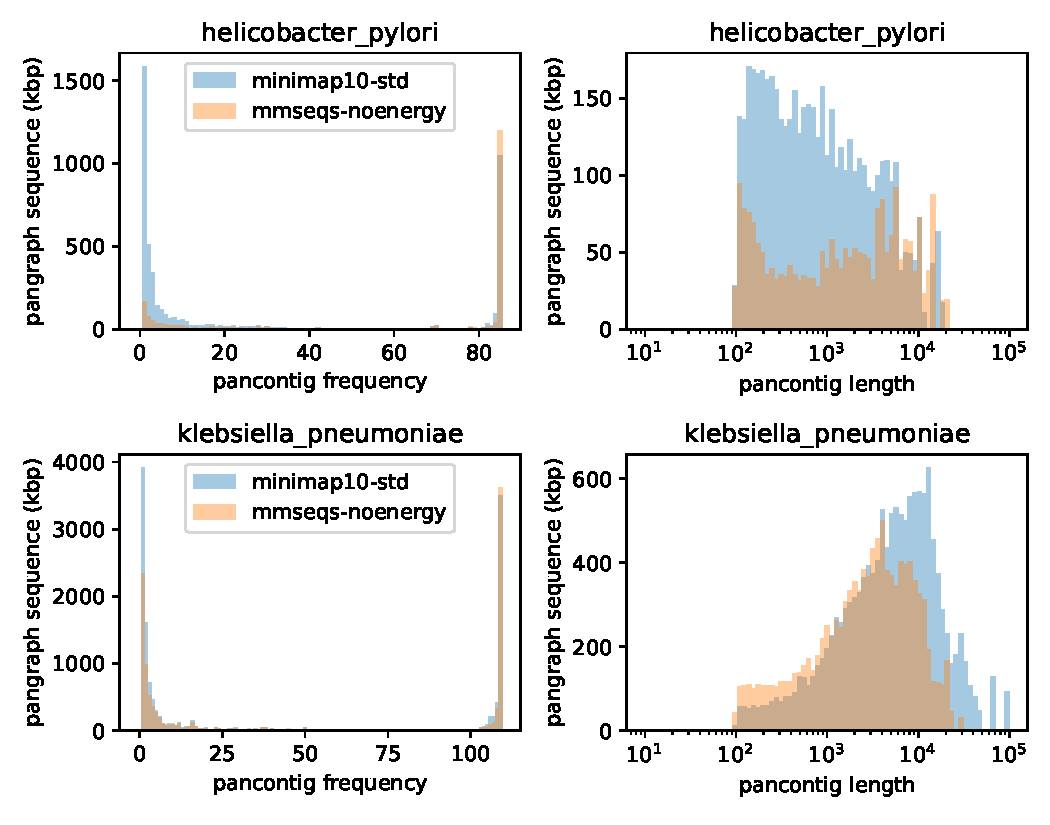
\includegraphics[width=.7\textwidth]{figs_response/hp_vs_kp.pdf}
      \caption{frequency and length distribution (respectively left and right panels) of pancontigs for the \textit{Helicobacter pylori} and \textit{Klebsiella pneumoniae} datasets (top and bottom). For each panel we report the results for pangenome graphs built using minimap2 aligner with standard parameter value and asm20 sensitivity (blue) and with mmseqs2 and null pseudo-energy parameters (orange). Distributions are weighed by pancontig length, so that the area under the curve represents the total pangenome graph size.}
      \label{fig:kp-vs-hp}
\end{figure}

\reviewer{R2.8}{Just to make sure i understand - is it possible for sequence to be ``left out'' in between pancontigs?}
\Marco{no, every part of the genome must be contained in a pancontig. It can be left out from the consensus if it is considered an insertion.}\\
\Liam{if they possibly misunderstood, suggests that some statement that all sequence ends up in a pancontig should be added to manuscript. I suspect they are thinking of case of short ($<$100bp) stretches `in between' pancontigs, which (if I understand correctly) will be incorporated as insertions at the end of the consensus alignment of the adjacent pancontig.}

\reviewer{R2.9}{About data accessibility
      \begin{enumerate}
            \item i don't see how to get the list of accessions for section IIB? Saying they were used in the Ding et al paper is not quite enough for me to be sure which ones you used.
            \item for the graph marginalisation section, could the accessions of the strains used be in a supplementary file as well as on github? Github repos are great, but they can be deleted.
      \end{enumerate}}
% \Marco{on the repo we have \href{https://github.com/neherlab/pangraph/blob/master/script/config/accnums.json}{this file} for the list of all accession numbers we use, and \href{https://github.com/neherlab/pangraph/blob/master/script/config/projection_strains.json}{this file} for the marginalization pairs. I could create some excel spreadsheet with accession numbers that we could add to the submission?}\\
% \Liam{for sure that's all they want (most biologists don't like json!)}
\responsedraft{We now included in the submission two excel files. ``accession\_numbers.xlsx'' contains five sheets, one per species considered, each with a list of the accession numbers of isolates used in our datasets. ``marginalize\_pairs.xlsx'' contains instead a list of all the pairs used in the graph marginalization section.
      % TODO: archive repository state.
}

\subsubsection*{Minor Issues}

\reviewer{R2.1}{line 13 - it would be good to give a reference for the statement that even closely related genomes can differ widely in gene content.
      I don't know what the first paper to show this was, the earliest i am aware of is from Eduardo Rocha's team, which annpoyingly i can't locate right now, but Figure 2 here shows it \url{https://journals.plos.org/plosgenetics/article?id=10.1371/journal.pgen.1008866} \cite{touchon2020phylogenetic} - you can be very close in patristic distance and have very different gene repertoire.
      Feel free to replace with a better reference, this si just meant to be helpful.}
\Marco{I think this is a good reference, fig. 2 is familiar to us. And also fig.2 in \cite{doolittle2009origin} which is a bit older. But not sure which other Rocha paper he is referring to.}\\
\Liam{I think they mean Figure 5 of \cite{touchon2009organised} (\href{https://journals.plos.org/plosgenetics/article?id=10.1371/journal.pgen.1000344}{here}). Citing Touchon 2009 and 2020 and the Doolittle paper seems fine to me.}

\reviewer{R2.2}{Why on earth is the "get an MSA of a block" option in pangraph called "polish"?}
\Marco{i don't think this comes from the paper (I used grep on the tex file and we never mention polish). I think it comes from the documentation but not sure where. We explain polish \href{https://neherlab.github.io/pangraph/tutorials/tutorial_3/\#Polishing-the-alignments}{in this part} of the tutorial and I don't think it's ambiguous. If in the paper we explain how we propagate the consensus sequence and related problems we will also mention the polish command in the same part and make explicit that it can be used to polish alignments, this should solve the ambiguity.}\\
\Liam{this sounds good. I think they misunderstood that polish is not just `extract the MSA' but actually produces a pangraph with the same structure but redone alignments. I think what is in the documentation there is great and could almost go straight in the paper, something like: `At each stage pancontigs are compared and aligned using their consensus sequences. This shortens considerably the time needed, but might introduce minor inconsistencies and artifacts in the alignments. These can be removed at the end of the process by reconstructing the sequences in the block and performing a multiple sequence alignment (see Polish command in documentation).')}

\reviewer{R2.3}{line 48: "Pancontigs are connected by an edge if they are syntenic on at least one input sequence;" - i think this is a bit of an abuse of modern language. The word syntenic is generally used to mean two genes/whatever have order conserved on multiple chromosomes (although some googling tells me that in classical genetics it meant things were on the same chromosome). Anyway, my understanding is pancontigs are connected by an edge if one of the input genomes is spelled out by going from one to the other. So it's about adjacency rather than synteny.}
% \Marco{I agree, we could use ``if they are ajacent/contiguous on at least one input sequence''?}\\
% \Liam{adjacent sounds good.}
\response{we agree with the reviewer observation. We modified ``syntenic on'' to ``adjacent in'' in line 48.}

\reviewer{R2.4}{Line 131: was N really=100? on the plot in figure 2, you have n.isolates going up to 1000}
% \Marco{$N=100$ was the standard value for the rest of the simulations (e.g. later for accuracy). I did a tentative correction: removed from the main the specification on population size and mentioned to check the SI for details on standard parameter values.}
\response{The value $N=100$ is the standard value used in the rest of the simulation, but as the reviewer pointed out this value is varied for the results showed in fig.~2 and the statement was confusing. We modified line 131 removing the value of $N$ and referring to SI section 1 for the standard value of simulation parameters.}

\reviewer{R2.5}{Figure 5 legend, lower case C in "coli" of "E. coli". Also italics.}
% \Marco{fixed.}
\response{The legend has been corrected.}


\reviewer{R2}{It is a bit depressing and unhelpful to structure a review only around problems and quibbles, so i wanted also to raise a number of
      Things I liked:

      \begin{enumerate}
            \item The paper is concise and well written, i really enjoyed reading it
            \item I liked the structure of the algorithms section, again i congratulate the authors, this is so much clearer than most papers. eg i was particularly happy to see the Guide Tree section start with your design constraints/aims.
            \item Fantastic choice of species in your empirical dataset - P. marinus diversity is insane.
            \item Line 215 - this is a remarkable achievement: "Adding more strains does not generate excessive fragmentation of these pancontigs, and their size remains of several kbps even as hundreds of strains are added"
            \item Congratulations
      \end{enumerate}
}


\subsection*{Reviewer 3}

\reviewer{R3}{The article "PanGraph: scalable bacterial pan-genome graph construction" reports a new method for constructing a Pan-Genome Graph (PGG) in an efficient manner with an open and extractable grah structure. Unfortunately, the authors appear to either be unaware of or downplay the existence of previous methods for the same purpose.\textbf{ The authors need to survey the existing literature and compare and contrast with their method to show the utility of their approach.}}

\reviewer{R3}{For instance the authors state: "Traditional computational approaches towards whole-genome analysis either scale poorly with the number of genomes, or treat genomes as dissociated "bags of genes", and thus are not suited for this new era.". There are many pan-genome analysis tools which treat the pan-genome as a graph and generate a PGG. There are two primary differences in these existing tools: those which generate a graph at the nucleotide level with nodes representing basepairs (sometimes nonbranching runs of nodes are collapsed) and those where nodes represent larger features such as genes.\\
      PanGraph appears to wed these approaches to some extent in that the alignments are done at the nucleotide level and the features are extracted as a characteristic of the alignments.}

\reviewer{R3}{An obvious lack in PanGraph is an attempt to map existing annotations back onto the generated PGG which is a necessity for usefulness to biologists. The mechanism for this is obvious but providing a useful user interface might be tedious.}
\Liam{I think perhaps producing a helper python script that converts a genbank annotation file for a genome within a pangraph to an output gff/csv with the block locations and coordinates would please this reviewer.}\\
\Marco{Yeah good idea. Maybe something that just map each annotation into a block, without solving the problem of harmonizing annotations which might be some more work...}\\

\reviewer{R3}{This statement: "While easy to conceptualize, the construction of pangenome graphs has proven computationally challenging. Colored generalizations of the de Bruijn graph-based assemblers have been successively used to build graphs from large sequence sets, although the underlying efficiency derives from a fixed k-mer size which prevents modelling long-range homology (Iqbal et al., 2012; Muggli et al., 2017)." appears to be incomplete at best. De Bruijn graph-based assemblers routinely collapse nonbranching portions of the graph into longer sequences than the k-mer size used for construction.
      % \Marco{from what I understand the structure in de Bruijn graphs is very fine-grained. Every SNP can generate a branching event. While in our case we have this intermediate corse-graining where homologous parts are collapsed together and the remaining structure of the graph represents large-scale structural variation in the genomes. I don't think this is solved by collapsing nonbranching portions in dB graphs (but I might not know enough about this...)}\\
      One early approach that does not explicitly generate a pan-genome graph but deals with some of the rearrangement issues cited by the authors is:
      \begin{itemize}
            \item \cite{angiuoli2011improving}
            \item \cite{angiuoli2011mugsy}
      \end{itemize}
      While the underlying approach is quite different, a very similar PGG to PanGraph is produced by a different method with similar nodes represented by multiple sequence alignments and edges with the same meaning:
      \begin{itemize}
            \item \cite{sutton2021pan}
            \item \cite{chan2015novel}
      \end{itemize}}

\reviewer{R3}{I believe this statement: "It is not uncommon that one pancontig has homology with multiple other pancontigs and the iterative algorithm has to make choice which potential mergers are performed and in which order." is the essential step in the process and perhaps deserves more focus. It captures two important issues: \textbf{aligning orthologs not paralogs and keeping the fracturing of the PGG nodes to a minimum}. The pseudo-energy captures the alignment length (longer is better for orthologs versus paralogs) but does not appear to capture the surrounding context of the iterative PGGs. For initial alignments of single genomes to single genomes this doesn't matter for the most part because there is a single pancontig for each each genome and PGG context is mostly captured in the alignment. I am not so sure this is true as the PGG nodes fracture and become much smaller. When choosing between competing mergers of paralogs/orthologs the context of the PGG and other possible mergers is important if the pancontigs have been reduced so that they contain only repetitive sequence without unique flaning sequence. I think this is a very important point as \textbf{distinguishing orthologs from paralogs is essential for correct PGG construction and the authors need to explicitly address it}. This could be measured as part of the simulated data where identical paralog sequences of various lengths and copy number could be modeled.}
\Liam{I am not sure I agree that constructing a pangenome graph means one must distinguish orthologs from paralogs. The structure is still useful even if this isn't done. Maybe there is a way of doing something of what they propose with simulations, but I suspect this isn't necessary for the editor to accept the paper\ldots}\\
\Marco{I agree, I think it's a different design choice. We could also mention that the marginalize command has an option to project out paralogs, but should be a post-processing step rather than something that we want to do while building the graph. One can a posteriori decide whether one wants to split paralogs using structural information (flanking blocks) or one can even prevent the merging using diversity and the $\beta$ parameter.}

\reviewer{R3}{In the pseudo-energy discussion a further parameter is mentioned: "In addition, there is parameter that controls the minimal size of contigs produced by the algorithm.". The value chosen for this parameter should be explicitly stated along with a rationale for the choice. It is also not clear if any of the splitting pancontigs are less than this value if the entire merger is dropped or just massaged to not have the too small new pancontig.}
\Liam{this relates to R2's point above about all sequence ending up in pancontigs so I think is just clarification.}\\
\Marco{I agree. We set a minimal cutoff of 100bp. This is stated later in line 106. Maybe we could expand the sentence in line 99 and give the value and few more words on the meaning/effect. This controls in some sense the ``corse graining'' of the graph: what is the size of an event that we want to encode as structural variation in the graph, rather than as an indel in the alignment. In the algorithm this minimal cutoff has different effects depending on the context. When aligning, if the match lenght is less than this threshold the merge is refused. For long alignments, if the CIGAR string contains indels that are longer than this threshold, these are saved as separate blocks and not as indels in the block. The same goes for the flanking sequences, if merging two long blocks leaves overhangs that are less than this threshold size then these overhangs are saved as part of the merged block and not as separate small blocks. This might be explained in the SI?}\\

\reviewer{R3}{How are pancontig consensus sequences determined and updated? I could not find any details about this. This is not a trivial operation. My reading of the article seems to imply that a complete multiple sequence alignment is not done for each merger. Does the consensus sequence degenerate iteratively with mergers? For the simulated data how accurate are the final pancontig consensus sequences?}
\Liam{expanding discussion of doing an MSA at end as for R2's comments would partially address. Quantifying how the consensus sequence degenerates iteratively is an interesting point that seems possible?}\\
\Marco{I agree, this could be addressed by adding a more detailed algorithm explanation of the merging algorithm in the SI. The short answer is that at each merging the full alignment is constructed using the CIGAR of the alignment of the consensus of the two blocks. Then consensus of the full alignment is re-evaluated. This does not solve the multiple alignment problem during constructions and there can be degeneration on where indels are mapped, but the final graph can be eventually polished. I don't think we ever quantified how much the consensus sequence degenerates during the iterations. Maybe one could devise a proper test set and see how it degenerates over the iterations.}

\reviewer{R3}{The statement: "Upon completion, transitive 108 edges within the graph, i.e., edges along which all path are co-linear, are removed by merging adjacent pancontigs." needs clarification. Why would these pancontigs have been split in the first place? Is there any necessary special issues with producing the merged multiple sequence alignment?}
\Liam{don't understand their last sentence. Maybe should quantify how common the transitive edges typically are?}\\
\Marco{I can think of one edge case which is due to periodic boundary conditions. Initially each circular genomes is saved as a single long block. If during alignment this unique blocks is split somewhere in the middle, the resulting edge blocks might be always colinear, since they are actually adjacent parts of the sequence that were artificially split to linearize the circular genome. One wants to collaps these two parts in a single block. This should happen often at the beginning of the merging of circular genomes. But might be unnecessary detail when explaining the algorithm the first time, we might want to move it to the SI section where we explain merging in more detail?}\\

\reviewer{R3}{It is not clear to me what Table 1 shows. Is this published data from PanX or data from PanGraph? Either way the value of 0.7 Mbp for the E. coli core genome length seems implausibly low for high quality complete genomes. The authors should justify this. The authors should also include analysis on the calculated core genome length versus actual core genome length for the simulated data.}
\Liam{0.7Mbp does seem lower than I would expect - I guess that they expect $>$2 Mbp - but it shows that obsessing about core is a bit unwise. With slightly relaxed definitions (95\% of genomes) does the core get sensibly bigger? For comparison e.g. ggCaller gets ~2,500 core genes in 100\% of n=162 \textit{E. coli} (Table 1 of \href{https://www.biorxiv.org/content/10.1101/2023.01.24.524926v1.full.pdf}{here}).}\\
\Marco{I checked and soft core (gene in 95\% of strains) is 2Mbp in our dataset. Some of our problems might come from weird strains. E.g. the second strain with the least amount of soft-core genes is \href{https://www.ncbi.nlm.nih.gov/nuccore/NC_020518.1?report=genbank}{NC\_020518}, an artificial genome that was removed from RefSeq. The strain that misses the most of the 1000 most frequent genes \href{https://www.ncbi.nlm.nih.gov/nuccore/NC_017663.1?report=genbank}{NC\_017663} was also removed from RefSeq. The rest might be due to misannotations? At least one of the most common 1000 genes are missed by 87/307 strains. Interestingly in \cite{sutton2021pan} they report $\sim$700 core orthologous gene clusters for an E.coli dataset of $\sim$1000 genomes, if they do not harmonize annotations. Those increase to $\sim$1500 after refining their annotations.\\
      The easiest thing to do might be to just add the size of soft-core for all species? Maybe these values might also be added as dashed lines in fig. 4G for comparison with pangraph's estimation?}\\
\reviewer{R3}{The authors might want to consider some form of post processing of the PGG to collapse what have been called bubbles in the graph if alignment of the pancontigs on different edges of the bubble warrant it.}
\Marco{if I understand correctly this is hinting at some form of post-processing step in which artifactual small blocks - generated at the edges of long block merges - could be absorbed in the flanking block alignments and removed?}\\

\reviewer{R3}{Overall the paper is well written. I like the basic methodology and the attention to using robust efficient existing algorithms and combining them to keep efficiency in mind. I am very concerned about the potential fracturing of the PGG where unfortunately the devil is in the details and am not convinced that the fracturing will not prevent some limit on the number of genomes which can be used for a pangenome.}
\Marco{if the fracturing derives from a real structural property of pangenomes (i.e. ISs that really move around and split long blocks) this might be an intrinsic limit that derives from the pangenome, I wouldn't consider it a problem with PanGraph.}\\

\reviewer{R3}{An issue I have struggled with in my own work is how to represent an orthologous gene cluster (node/vertex) within the PGG when the gene sequence in some genomes has an insertion event such as an IS element within the gene. I assume for PanGraph that this would necessitate splitting the node into multiple pancontigs. How is this sustainable for species with large numbers of active IS elements? This could also be investigated for PanGrah using suitable simulated data.}
\Liam{I think nothing to say here apart from `yes, active IS elements split pancontigs up' (and can themselves be split up due to similarity with other IS\ldots). For the future one might want to have pangenome methods where you can explicitly pass a list of predefined sequences that should not be split. But I think this is a general problem and not something to investigate with simulations or fix here.}\\
\Marco{agree. I think this is a structural property that we want to capture, the fact that these pancontigs are split.}


\bibliography{cite}{}

\end{document}

% meeting notes:
% SIAS -> (new) Supplementary Information Algorithm Section
% make changes in the text traceable in the reviewer answers.
% Reviewer 1:
% - for blocks, mention that consensus is considered as the centroid of a star-shaped phylogeny?
% - 2) add line to fig. on compression
% - 5) the effect comes from the fact that core genes are in long syntenic stretches, compared to accessory that are often in messy islands (cite Rocha?). Just add half sentence to the paper.
% - 6) annotate the figure with numbers
% - 8) reference: graph alighner, ggCaller? Many take GFA as input.\
% - 10) this is something that could be explained in the SIAS: one starts with long and shallow blocks and as graphs are merged and propagated down the tree the blocks become shorter and deeper. Removing energy threshold just causes more merging and deeper but shorter blocks. (figure?)
% - test pangraph with 500 E.coli.
% Reviewer 2:
% - 1) do not mention blocks, only pancontigs
% - specify better the meaning of null energy parameters and why more merging.
% Reviewer 3:
% - paralog merging is partially controlled by beta. As future direction one should build trees for every blok and split paralogs in a PanX fashion. 
% - more nuanced treatment of the literature.
% - update marginalize figure legend
% - update SI section numbering in the main text